% example tikz figure

\documentclass{article}

\usepackage{tikz}
\usetikzlibrary{arrows,shapes,positioning,shadows,trees}


\begin{document}

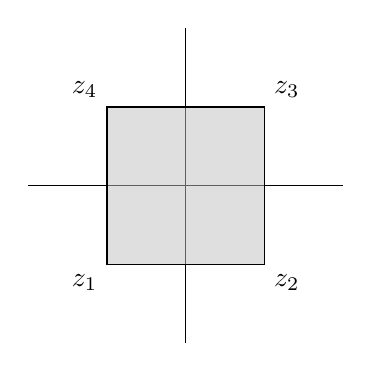
\begin{tikzpicture}
  % draw axis with no labels, size 4x4
  \draw[-] (-2,0) -- (2,0);
  \draw[-] (0,-2) -- (0,2);

  % draw a square centered at the origin with side length 2, fill gray with 50% opacity
  \fill[gray!50,opacity=0.5] (-1,-1) rectangle (1,1);

  % stroke the square above
  \draw (-1,-1) rectangle (1,1);

  % label the corners of the square, using the anchor points
  \node[anchor=north east] at (-1,-1) {$z_1$};
  \node[anchor=north west] at (1,-1) {$z_2$};
  \node[anchor=south west] at (1,1) {$z_3$};
  \node[anchor=south east] at (-1,1) {$z_4$};
\end{tikzpicture}

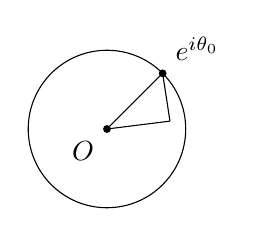
\begin{tikzpicture}
  % draw cicrle with radius 1, centered at the origin
  \draw (0,0) circle (1);

  % label (0,0) with a dot, captioned O at bottom left
  \node[fill,circle,inner sep=1pt,label=below left:$O$] at (0,0) {};

  % label (\sqrt{2} / 2, \sqrt{2} / 2) with a dot, captioned $e^{i\theta_0}$ at top right
  \node[fill,circle,inner sep=1pt,label=above right:$e^{i\theta_0}$] at (0.707,0.707) {};

  % connect the two dots with a line
  \draw (0,0) -- (0.707,0.707);

  % draw a line that starts from the theta_0 with angle theta from its line to the origin
  \draw (0.707,0.707) -- (0.8,0.1);
  \draw (0,0) -- (0.8,0.1);
\end{tikzpicture}

\end{document}